\documentclass[11pt,a4paper]{article}
\usepackage[utf8]{inputenc}
\usepackage[T1]{fontenc}
\usepackage{lmodern}
\usepackage{textcomp}
\usepackage{amsmath,amssymb}
\usepackage{graphicx}
\usepackage{booktabs}
\usepackage{longtable}
\usepackage{array}
\usepackage{listings}
\usepackage{xcolor}
\usepackage[margin=1in]{geometry}
\usepackage{float}
\usepackage[hidelinks,breaklinks]{hyperref}
\usepackage{microtype}
\setlength{\parskip}{4pt}
\lstset{basicstyle=\ttfamily\scriptsize,breaklines=true,breakatwhitespace=false,
  postbreak=\mbox{\textcolor{gray}{$\hookrightarrow$}\space},frame=single,
  framerule=0.3pt,rulecolor=\color{gray!60},columns=fullflexible,keepspaces=true,
  showstringspaces=false,numbers=none,xleftmargin=4pt,xrightmargin=4pt,
  literate={\_}{{\_}}1}
\graphicspath{{figures/}}
\providecommand{\tightlist}{}
\title{Lyman-alpha Warm Dark Matter Limits Compared with Dodelson-Widrow Sterile-Neutrino Production Fractions}
\author{HEP-Genesis-Agent session record \\ \small Project: ramp-research-lyman-wdm}
\date{2026-10-19}
\begin{document}
\maketitle
\noindent\textit{\small This document is an AI-generated account of an interactive session with the HEP-Genesis agent. Its text was written by a language model strictly from the session record; figures and numbers come only from tool results obtained during the session. The supplementary material and the transcript, generated alongside, document exactly what ran. Verify independently before use.}
\vspace{1em}

\begin{abstract}
We report a literature-and-tool study that compares recent high-redshift Lyman-$\alpha$ forest constraints on warm dark matter (WDM) with non-resonant (Dodelson-Widrow, DW) production of keV sterile neutrinos. Thermal-relic lower limits were checked against the papers: $m_{\rm WDM}>5.7$ keV (95\% CL) from arXiv:2309.04533, which drops to 4.1 keV when the analysis is restricted to $k_{\max}<0.1$ s/km with earlier thermal-history priors; 3.1 keV from arXiv:2209.14220; and 3.3 keV from arXiv:1306.2314. Only the first was checked against its full text. We verified the Viel et al.\ 2005 mapping (astro-ph/0501562, Eq.~5) against its full text and used it to convert these limits to DW mass floors of 20.2, 21.9, 29.3 and 45.4 keV for $\omega_{\rm dm}=0.12$. A sterile-neutrino tool server returned DW relic abundances that scale linearly with $\sin^2 2\theta$. Rescaling them gives the mixing at which DW sterile neutrinos are all of the dark matter ($f_s=1$): $3.95\times10^{-11}$, $3.32\times10^{-11}$, $2.02\times10^{-11}$ and $9.17\times10^{-12}$ at 20, 22, 29 and 45 keV. At the 3.5 keV line point the tool gives $f_s=0.275$. Two published DW yield fits require 3 to 16 times larger mixing for the same abundance, so the production fraction is uncertain by that factor; this comparison is contested. The tool's coarse X-ray check excludes $f_s=1$ at 20 keV. It has no coverage at 29 and 45 keV. No numerical X-ray limits on $\sin^2 2\theta$ were extracted, so the maximum X-ray-allowed DW fraction at each Lyman-$\alpha$ floor could not be computed. On the evidence gathered, the session did not demonstrate that 100\% DW dark matter is excluded by combined Lyman-$\alpha$ and X-ray data. It did collect published statements to that effect, quoted verbatim.
\end{abstract}

\section{Introduction}
The user asked for three things: a survey of recent Lyman-$\alpha$ forest constraints on warm dark matter; a comparison of those constraints with sterile neutrinos produced non-resonantly (Dodelson-Widrow); and the use of the available sterile-neutrino tools to compute production fractions $f_s=\Omega_s/\Omega_{\rm dm}$.

The session split this into five lines of work:
\begin{enumerate}
\item DW relic abundance and $f_s$ across the $(m_s,\sin^2 2\theta)$ plane from the tool server.
\item Verification of the thermal-relic Lyman-$\alpha$ limits and of the cold-plus-warm (mixed) bounds on the warm fraction.
\item Verification of the thermal-relic-to-DW mass mapping and of alternative mappings.
\item Numerical X-ray upper limits on $\sin^2 2\theta$ over roughly 5--50 keV, added at the critic's request.
\item A cross-check of the tool's DW normalisation against published yield formulas, and a final comparison table.
\end{enumerate}
The first two were completed. The last three were left blocked, for reasons described below.

The scope is restricted to tool outputs and to the paper texts read during the session. No Boltzmann-code transfer functions or new Lyman-$\alpha$ likelihoods were computed.

\section{Methods}
\paragraph{Execution and tools.}
All work ran with local dispatch. Three groups of tools were used:
\begin{itemize}
\item a literature toolset: arXiv abstract search, arXiv API search, metadata retrieval, full-text download, chunked text reading, figure extraction from arXiv HTML, citation recording and web search;
\item a sterile-neutrino server described as a ``Sterile Neutrino $\to$ BBN / X-ray Bridge Server'';
\item a research board for recording findings, dead ends and questions.
\end{itemize}

\paragraph{Sterile-neutrino server.}
The server maps $(m_s,\sin^2 2\theta,\text{mechanism})$ to $\Delta N_{\rm eff}$, $\Omega_s h^2$, a radiative-decay line, a free-streaming length and BBN observables. Its BBN treatment fits $Y_p$, D/H and $^7$Li to the PRyMordial network to within $0.3\%$. A point counts as BBN-excluded when $\Delta\chi^2$ relative to the Standard Model exceeds 3.84 (95\%, 1 dof). This treatment is stated to be valid for $m_s\lesssim 100$ keV.

The loaded skill recipe gives the decay rate as
\[
\Gamma=1.36\times10^{-32}\,{\rm s^{-1}}\,\frac{\sin^2 2\theta}{10^{-10}}\left(\frac{m_s}{\rm keV}\right)^5,
\]
with line energy $E_\gamma=m_s/2$. A point overcloses when $\Omega_s h^2>0.12$. The X-ray check computes whole-halo fluxes for five targets (Milky Way centre, M31, Coma, Perseus, stacked galaxies), assuming $f_{\rm DM}=1$ and no field-of-view cut. It reports only whether a tabulated limit lying within 30\% in mass excludes the point.

\paragraph{Calculations run.}
\begin{itemize}
\item A single DW point at $(7.1\ {\rm keV},\ 7\times10^{-11})$.
\item A DW grid of 17 masses (1--100 keV) by 22 mixings ($10^{-13}$--$10^{-6}$), 374 points in total.
\item A 12-point grid at $\sin^2 2\theta=10^{-12}$ for 7.1--100 keV.
\item A DW plane scan of $80\times80=6400$ points over $m_s=1$--100 keV and $\sin^2 2\theta=10^{-14}$--$10^{-6}$, with its exclusion plot.
\item X-ray line checks at 20, 29 and 45 keV at the respective $f_s=1$ mixings.
\end{itemize}
The mixing at $f_s=1$ was obtained by linear rescaling of $\Omega_s h^2$ to 0.12. This rescaling, the DW mass floors, the half-mode estimates and the comparisons with published yield fits are the assistant's hand arithmetic, not tool outputs.

\paragraph{Literature.}
Full texts were downloaded and partly read for arXiv:2309.04533, 2504.06367, 0812.0010, 1609.00667, 1908.09037, 2207.04572, 1702.08430, 2007.13751, astro-ph/0501562, astro-ph/0511630 and hep-ph/0612182. astro-ph/0512631 was downloaded but not read. One read of 1908.09037 failed with a UTF-8 decoding error. A web search for an alternative thermal-to-DW relation returned nothing. Figure extraction returned two figures for arXiv:2504.06367 and eleven for arXiv:0812.0010.

\section{Results}
\subsection{Survey of Lyman-$\alpha$ thermal-relic limits}
Table~\ref{tab:lya} summarises the limits gathered. Only the arXiv:2309.04533 numbers were checked against the full text; the others come from retrieved abstracts.

\begin{table}[h]
\centering
\begin{tabular}{llll}
\toprule
Paper & Data & Limit (95\% CL / $2\sigma$) & Check \\
\midrule
arXiv:2309.04533 & HIRES+UVES, $z=4.2$--5.0, $k_{\max}=0.2$ s/km & $>5.7$ keV & full text \\
arXiv:2309.04533 & restricted, $k_{\max}<0.1$ s/km, earlier priors & $>4.1$ keV & full text \\
arXiv:2209.14220 & 1080 Cholla sims vs.\ Boera+2019, $4.0\lesssim z\lesssim5.2$ & $>3.1$ keV (peak 4.5 keV) & abstract \\
arXiv:1306.2314 & 25 HIRES/MIKE quasars, $z>4$ & $>3.3$ keV & abstract \\
arXiv:1702.01764 & XQ-100 alone; HIRES/MIKE; combined & 1.4; 4.1; 5.3 keV & abstract \\
\bottomrule
\end{tabular}
\caption{Thermal-relic WDM mass lower limits collected in the session.}
\label{tab:lya}
\end{table}

The main stated systematics in arXiv:2309.04533 are IGM peculiar-velocity structure and inhomogeneous reionization. The paper says the thermal-history uncertainty now matters less. The 1080-simulation analysis (arXiv:2209.14220) reports that the WDM suppression saturates at $k>0.1$ s/km because of peculiar-velocity smearing.

For arXiv:1702.01764, the assistant's report adds that the combined 5.3 keV assumes a power-law $T(z)$, and that it relaxes to 3.5 keV if temperature jumps of 5000 K are allowed. The assistant also listed a historical $\sim$0.75 keV limit from Narayanan et al.\ 2000 (astro-ph/0005095). That value was not shown in any retrieved text.

\subsection{Mixed cold-plus-warm bounds}
Garcia-Gallego et al.\ (arXiv:2504.06367) used Sherwood-Relics simulations with a neural-network emulator and UVES+HIRES data at $z=4.2$--5.0. They give $f_{\rm WDM}<0.16$, 0.35, 0.50 and 0.67 ($2\sigma$) at thermal-relic masses of 1, 2, 3 and 4 keV.

Boyarsky et al.\ (arXiv:0812.0010) used WMAP5 with SDSS and VHS Lyman-$\alpha$ data. They express their bounds directly in the non-resonantly produced mass $m_{\rm nrp}$. In the pure-WDM case they find $m_{\rm nrp}\ge 8$ keV (frequentist 99.7\%) or 12.1 keV (Bayesian 95\%). Any $m_{\rm nrp}>5$ keV is allowed if $F_{\rm wdm}<0.6$ (99.7\%) or $F_{\rm wdm}<0.35$ (Bayesian 95\%).


\begin{figure}[H]
\centering
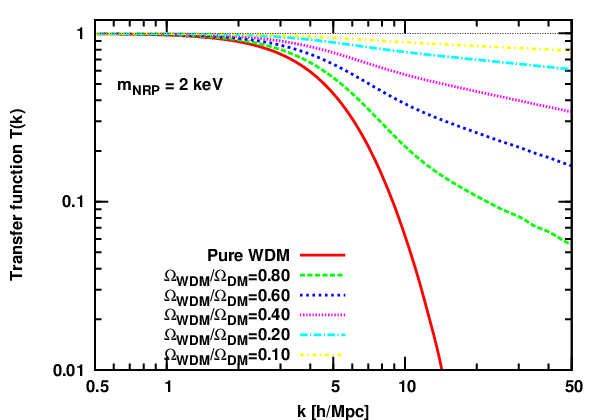
\includegraphics[width=0.85\textwidth,height=0.6\textheight,keepaspectratio]{fig-10.png}
\caption{Figure 1: Transfer functions T(k)\textbackslash{}equiv\textbackslash{}left[\{P\_\{\textbackslash{}Lambda\{\textbackslash{}textsc\{cwdm\}\}\}(k)\}/\{P\_\{\textbackslash{}Lambda\{\textbackslash{}textsc\{cdm\}\}\}(k)\}\textbackslash{}right]\textasciicircum{}\{1/2\} for m\_\{\textbackslash{}textsc\{nrp\}\}=2\textasciitilde{}\textbackslash{}mathrm\{keV\} and different WDM fractions: from left to right, \textbackslash{}Omega\_\{\textbackslash{}textsc\{wdm\}\}/(\textbackslash{}Omega\_\{\textbackslash{}textsc\{wdm\}\}+\textbackslash{}Omega\_\{\textbackslash{}textsc\{cdm\}\})=1,0.8,0.6,0.4,0.2,0.1. Other parameters are fixed to \textbackslash{}Omega\_\{\textbackslash{}textsc\{b\}\}=0.05, \textbackslash{}Omega\_\{\textbackslash{}textsc\{m\}\}=0.3, \textbackslash{}Omega\_\{\textbackslash{}Lambda\}=0.7, h=0.7. [arXiv:0812.0010] Reproduced from arXiv:0812.0010 (extracted with \texttt{get\_paper\_figures}).}
\label{fig:10}
\end{figure}



Figure~\ref{fig:10}, from arXiv:0812.0010, shows transfer functions for $m_{\rm nrp}=2$ keV at warm fractions from 1 down to 0.1. The point is that in mixed models the suppression becomes a partial step rather than a full cutoff.


\begin{figure}[H]
\centering
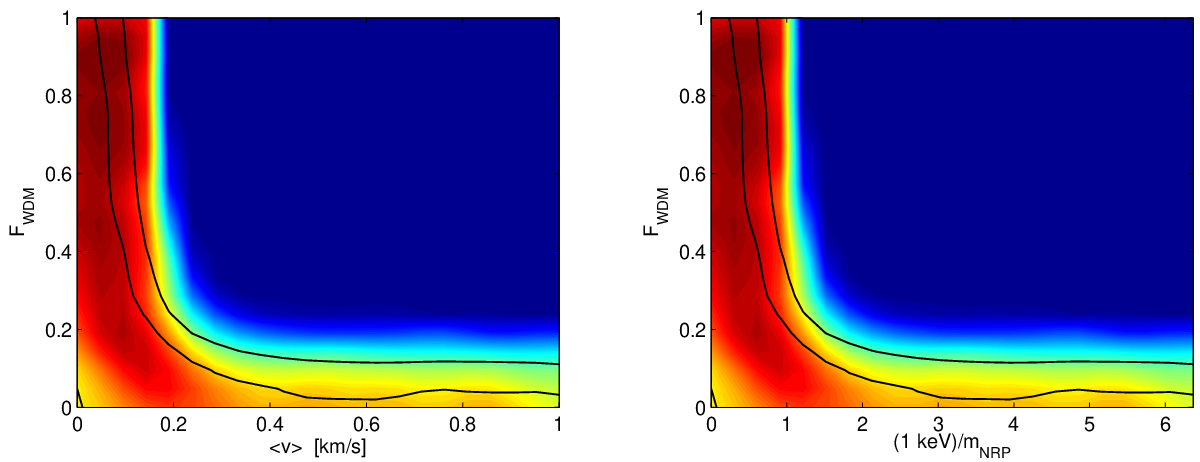
\includegraphics[width=0.85\textwidth,height=0.6\textheight,keepaspectratio]{fig-17.png}
\caption{Figure 7: (Left) Preferred region for the parameters (\{F\_\{\textbackslash{}textsc\{wdm\}\}\},\textbackslash{}langle v\textbackslash{}rangle\_\{\textbackslash{}textsc\{wdm\}\}) of the \textbackslash{}LambdaCWDM model, using VHS, WMAP5 and other cosmological data sets. The black lines represent the 68\textbackslash{}\%CL and 95\textbackslash{}\%CL contours of the two-dimensional probability marginalized over other parameters (as defined in the Bayesian approach), while the colors show the likelihood averaged over other parameters. (Right) Same plot with the horizontal axis translated in terms of (1\textbackslash{}mathrm\{keV\}/m\_\{\textbackslash{}textsc\{nrp\}\})=\textbackslash{}langle v\textbackslash{}rangle\_\{\textbackslash{}textsc\{wdm\}\}/(157\textasciitilde{}\textbackslash{}mathrm\{m/s\}), see equation (29). [arXiv:0812.0010] Reproduced from arXiv:0812.0010 (extracted with \texttt{get\_paper\_figures}).}
\label{fig:17}
\end{figure}



Figure~\ref{fig:17}, also from arXiv:0812.0010, shows the preferred $(F_{\rm wdm},\langle v\rangle_{\rm wdm})$ region from VHS, WMAP5 and other data. Its right panel converts the horizontal axis to $1\,{\rm keV}/m_{\rm nrp}=\langle v\rangle_{\rm wdm}/(157\ {\rm m/s})$. This is the constraint in the form needed to bound the DW fraction at a given mass.


\begin{figure}[H]
\centering
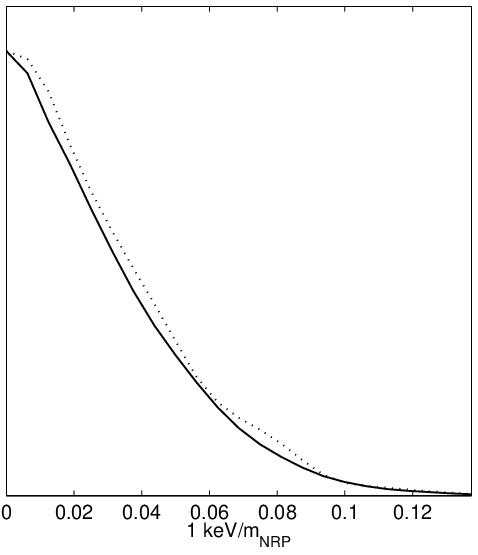
\includegraphics[width=0.85\textwidth,height=0.6\textheight,keepaspectratio]{fig-19.png}
\caption{Figure 9: Probability distribution for the parameter 1\textbackslash{},\textbackslash{}mathrm\{keV\}/m\_\{\textbackslash{}textsc\{nrp\}\} (which is identical to \textbackslash{}langle v\textbackslash{}rangle\_\{\textbackslash{}textsc\{wdm\}\}/(157\textasciitilde{}\textbackslash{}mathrm\{m/s\})) in the pure \textbackslash{}LambdaWDM case, using WMAP5 and SDSS Ly-\textbackslash{}alpha data, and starting from a flat prior on this parameter; the solid line shows the marginalized posterior, while the dashed line shows for comparison the average likelihood. The normalization of the y-axis (the probability) is arbitrary. [arXiv:0812.0010] Reproduced from arXiv:0812.0010 (extracted with \texttt{get\_paper\_figures}).}
\label{fig:19}
\end{figure}




\begin{figure}[H]
\centering
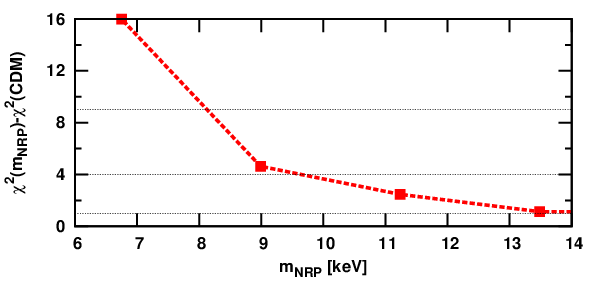
\includegraphics[width=0.85\textwidth,height=0.6\textheight,keepaspectratio]{fig-20.png}
\caption{Figure 10: Dependence of \textbackslash{}Delta\textbackslash{}chi\textasciicircum{}\{2\}=-2\textbackslash{}log\textbackslash{}mathcal\{L\} on the WDM mass m\_\{\textbackslash{}textsc\{nrp\}\}. The values are taken from Table 2, and the dashed line linearly interpolates between the points. [arXiv:0812.0010] Reproduced from arXiv:0812.0010 (extracted with \texttt{get\_paper\_figures}).}
\label{fig:20}
\end{figure}



The pure-WDM case is shown in Figure~\ref{fig:19} and Figure~\ref{fig:20}, again from arXiv:0812.0010. The first is the posterior of $1\,{\rm keV}/m_{\rm nrp}$ from WMAP5 and SDSS; the second is $\Delta\chi^2$ as a function of $m_{\rm nrp}$, taken from that paper's Table 2. Together they underlie the 8 and 12.1 keV pure-DW floors.

The constraint plots of arXiv:2504.06367 could not be extracted. The arXiv HTML returned only a density slice and an emulator schematic, so the mixed-DM curve could not be digitised.

The assistant mapped the 1--4 keV thermal masses of arXiv:2504.06367 to DW masses of about 4.4, 11, 18 and 28 keV. This is its own estimate using the Viel relation.

\subsection{Thermal-relic to DW mapping}
Viel et al.\ 2005 (astro-ph/0501562), Eq.~(5), was verified in the full text:
\[
m_{\rm sterile}=4.43\ {\rm keV}\left(\frac{m_{\rm thermal}}{1\ {\rm keV}}\right)^{4/3}\left(\frac{0.25\,(0.7)^2}{\omega_x}\right)^{1/3}.
\]
It is derived by equating $\omega_x$ and $m_x/T_x$ for a thermal relic and for a sterile neutrino ``which share the same phase-space distribution but with an overall suppression factor $\chi$''. The DW spectrum is therefore treated as a rescaled Fermi-Dirac distribution, and the two transfer functions are identical by construction.

This removes a caveat from the opening survey, where the assistant had quoted the relation from memory. The resulting DW floors are given in Table~\ref{tab:floors}. They agree with the survey's rough values of 20, 22, 29 and 45 keV to within 1\%.

\begin{table}[h]
\centering
\begin{tabular}{ccc}
\toprule
$m_{\rm WDM}$ limit & DW floor, $\omega_{\rm dm}=0.12$ & DW floor, $\omega=0.1225$ \\
\midrule
3.1 keV & 20.2 keV & 20.0 keV \\
3.3 keV & 21.9 keV & 21.8 keV \\
4.1 keV & 29.3 keV & 29.1 keV \\
5.7 keV & 45.4 keV & 45.1 keV \\
\bottomrule
\end{tabular}
\caption{DW mass floors from the verified Viel 2005 relation (assistant arithmetic).}
\label{tab:floors}
\end{table}

The Viel fit is $T(k)=[1+(\alpha k)^{2\nu}]^{-5/\nu}$ with $\nu=1.12$, calibrated for $k<5\,h$/Mpc. For thermal relics,
\[
\alpha=0.049\,(m_x/{\rm keV})^{-1.11}(\Omega_x/0.25)^{0.11}(h/0.7)^{1.22}\,h^{-1}\,{\rm Mpc}.
\]
The assistant derived $k_{\rm hm}=0.325/\alpha$ from the half-mode condition. This gives $\alpha=0.01396$, 0.01302, 0.01024 and $0.00710\,h^{-1}$ Mpc, and hence $k_{\rm hm}\approx23.3$, 25.0, 31.8 and $45.8\,h$/Mpc, for the four limits.

The critic contested this result. The values lie far outside the fit's calibrated range and were not compared with the half-mode mass quoted in arXiv:1306.2314. Under the Viel mapping they also cannot test the mapping itself, since the DW and thermal $k_{\rm hm}$ coincide by construction.

The framework of arXiv:2007.13751 uses $T(k)=[1+(\alpha k)^\beta]^\gamma$. This reduces to the Viel form for $\beta=2\nu$ and $\gamma=-5/\nu$, and fits a 2 keV WDM with $[\alpha,\beta,\gamma]=[0.02,2.2,-4.5]$. In the sections read it gives no DW-specific relation. No second mapping was verified.

\subsection{DW production fractions from the tool}
Contrary to the warning in the opening survey that no production-fraction tool was available, the server returned DW $\Omega_s h^2$ directly. It assumes pure DW production, with resonant (Shi-Fuller) production as a separate option.

$\Omega_s h^2$ scales linearly with $\sin^2 2\theta$ across the 374-point grid. Table~\ref{tab:fs} lists the tool values at $\sin^2 2\theta=10^{-12}$ and the rescaled $f_s=1$ mixings.

\begin{table}[h]
\centering
\begin{tabular}{cccc}
\toprule
$m_s$ & $\Omega_s h^2$ at $10^{-12}$ & $\lambda_{\rm fs}$ [kpc] & $\sin^2 2\theta(f_s=1)$ \\
\midrule
7.1 keV & 0.000471462 & 151.4 & $2.55\times10^{-10}$ \\
20 keV & 0.00304114 & 53.7 & $3.95\times10^{-11}$ \\
22 keV & 0.00361029 & 48.9 & $3.32\times10^{-11}$ \\
29 keV & 0.00593606 & 37.1 & $2.02\times10^{-11}$ \\
45 keV & 0.0130907 & 23.9 & $9.17\times10^{-12}$ \\
\bottomrule
\end{tabular}
\caption{Tool DW abundances and free-streaming lengths, with the mixing rescaled to $f_s=1$.}
\label{tab:fs}
\end{table}

At the 3.5 keV line point $(7.1\ {\rm keV},\,7\times10^{-11})$ the tool returns $\Omega_s h^2=0.033$, i.e.\ $f_s=0.275$. It also gives $E_\gamma=3.55$ keV, $\tau_\gamma=5.82\times10^{27}$ s and $\Delta N_{\rm eff}=4.3\times10^{-4}$, with BBN $\Delta\chi^2=-0.01$ (allowed).

\subsection{BBN in the DW plane}
The 6400-point scan found 3092 overclosing points and 968 BBN-excluded points. The largest BBN-allowed mixing falls from $3.93\times10^{-7}$ at 1 keV to $3.03\times10^{-8}$ at 26.2 keV, $1.5\times10^{-8}$ at 49.7 keV and $9.43\times10^{-9}$ at 100 keV. This is roughly three orders of magnitude above the $f_s=1$ line, so BBN does not constrain DW dark matter in this range.


\begin{figure}[H]
\centering
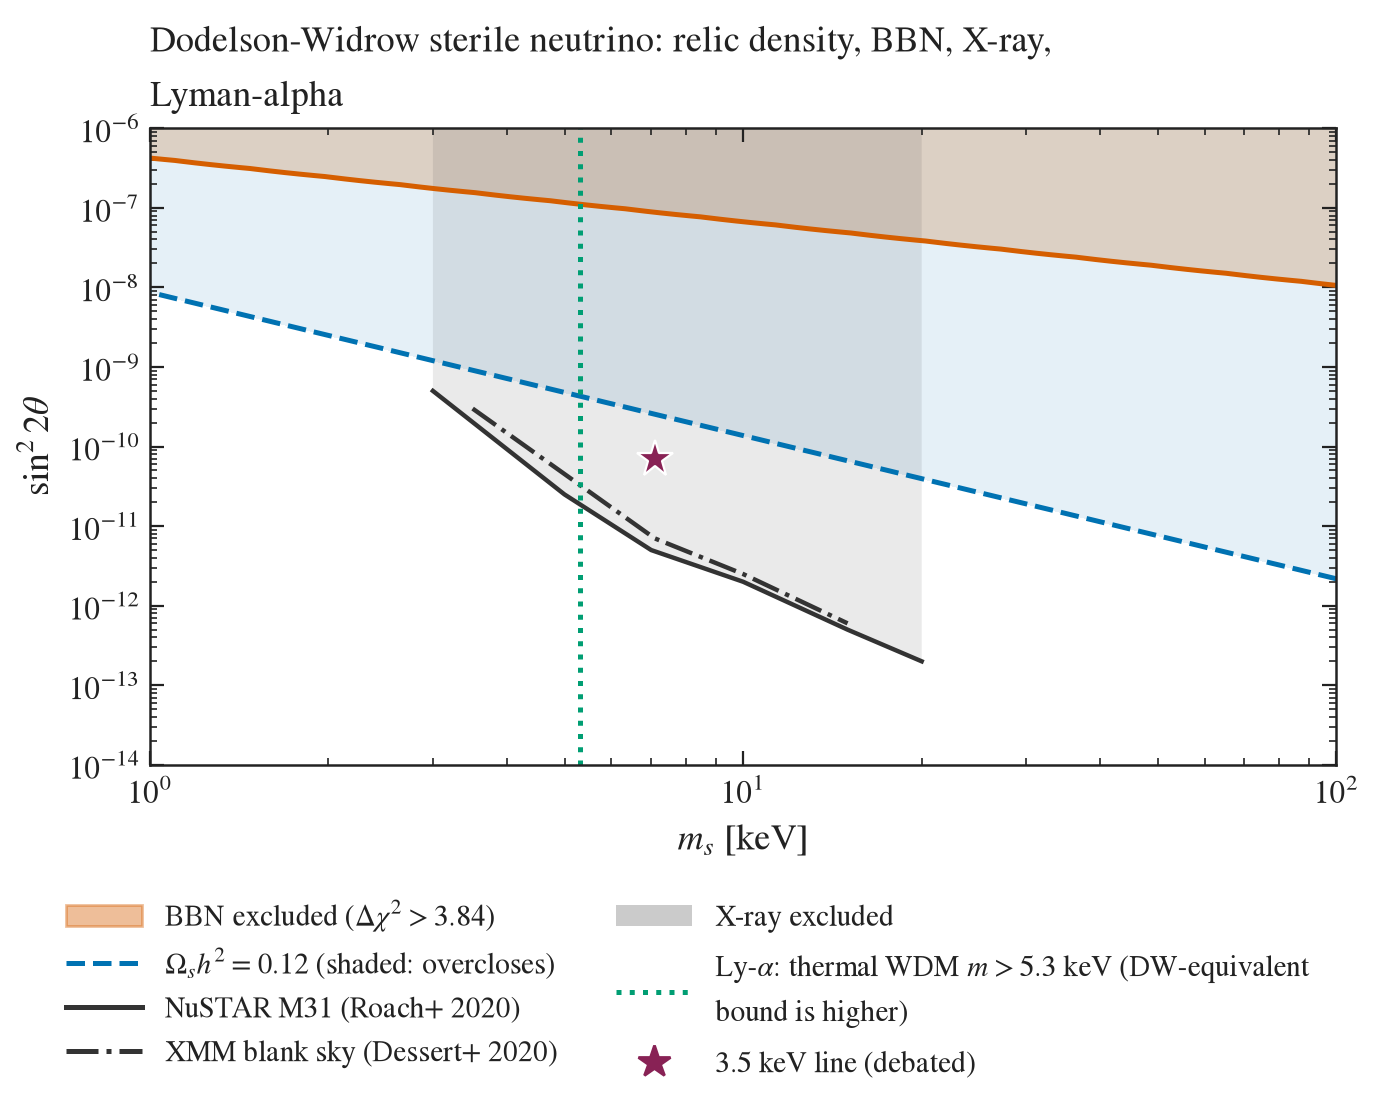
\includegraphics[width=0.85\textwidth,height=0.6\textheight,keepaspectratio]{fig-25.png}
\caption{exclusion\_scan\_DW\_d94a06.png Produced in this session by \texttt{plot\_sterile\_nu\_exclusion} on \textit{serve-sbbn.sh}.}
\label{fig:25}
\end{figure}



Figure~\ref{fig:25} shows the tool's DW exclusion plane from this scan, titled ``relic density, BBN, X-ray, Lyman-alpha''. Physically, the overclosure boundary, not BBN, sets the relevant upper edge of the mixing. The decisive comparison is therefore between the $f_s=1$ line, the X-ray limits and the Lyman-$\alpha$ mass floors.

\subsection{Cross-check of the DW normalisation (contested)}
Two published fits were read in full text. Their quotes were not formally recorded with the citation tool before the budget ran out.

The first is Abazajian 2006 (astro-ph/0511630), Eq.~7, for $T_{\rm QCD}=170$ MeV and electron flavour:
\[
m_s=3.40\ {\rm keV}\,(\sin^2 2\theta/10^{-8})^{-0.615}(\Omega_{\rm DM}/0.26)^{0.5}.
\]
The second is the ``most conservative'' line of Asaka, Laine and Shaposhnikov (hep-ph/0612182, Sec.~7.1):
\[
\log_{10}\sin^2 2\theta=-7.6195-1.7428\log_{10}(M/{\rm keV}).
\]
That paper states this line for $M\le4$ keV, so its use here is an extrapolation.

Inverting both fits gives the $f_s=1$ mixings in Table~\ref{tab:norm}. They exceed the tool's values by factors of 11.9--16.4 (Abazajian) and 3.10--3.44 (Asaka-Laine-Shaposhnikov). The tool therefore produces 3 to 16 times more DW dark matter per unit mixing.

At the 3.5 keV point, $f_s$ becomes 0.275 (tool), 0.089 (Asaka-Laine-Shaposhnikov) or 0.023 (Abazajian). The critic contested both the factor and its downstream use. It asked that the factor be settled with a modern DW calculation valid at 10--50 keV.

\begin{table}[h]
\centering
\begin{tabular}{cccc}
\toprule
$m_s$ & Tool & Abazajian 2006 (ratio) & ALS (ratio) \\
\midrule
7.1 keV & $2.55\times10^{-10}$ & $3.02\times10^{-9}$ (11.9) & $7.88\times10^{-10}$ (3.10) \\
20 keV & $3.95\times10^{-11}$ & $5.61\times10^{-10}$ (14.2) & $1.30\times10^{-10}$ (3.29) \\
22 keV & $3.32\times10^{-11}$ & $4.80\times10^{-10}$ (14.4) & $1.10\times10^{-10}$ (3.31) \\
29 keV & $2.02\times10^{-11}$ & $3.06\times10^{-10}$ (15.2) & $6.79\times10^{-11}$ (3.36) \\
45 keV & $9.17\times10^{-12}$ & $1.50\times10^{-10}$ (16.4) & $3.16\times10^{-11}$ (3.44) \\
\bottomrule
\end{tabular}
\caption{$\sin^2 2\theta(f_s=1)$ under three normalisations (assistant arithmetic; contested).}
\label{tab:norm}
\end{table}

\subsection{X-ray status of the $f_s=1$ points}
\paragraph{Tool checks.} The tool's check flagged 20 keV at $\sin^2 2\theta=3.95\times10^{-11}$ ($E_\gamma=10$ keV, $\tau=5.81\times10^{25}$ s) as excluded by its tabulated ``NuSTAR M31 (Roach+ 2020)'' point. At 29 keV ($2.02\times10^{-11}$) and 45 keV ($9.17\times10^{-12}$) it reported ``not excluded''. That flag only means no tabulated limit lies within 30\% in mass, so these masses are not covered rather than allowed. The 22 keV case was not run. The critic contested this finding because it rests on the tool's sparse tabulation.

\paragraph{Literature statements.} The following quotes were verified:
\begin{itemize}
\item Perez et al.\ (arXiv:1609.00667): ``In most of the mass range 10--50 keV, these are now the strongest limits, at some masses improving upon previous limits by a factor of $\sim$ 10''.
\item Roach et al.\ 2020 (arXiv:1908.09037) report no anomalous lines at 5--20 keV, i.e.\ $m_s=10$--40 keV. Their limits are given on $\Gamma$, plotted from $10^{-29}$ to $10^{-27}$ s$^{-1}$. The paper says they improve on earlier limits by about $2\times$ at 10--12 keV and are weaker near 16 and 30--40 keV. This reading is contested.
\item Roach et al.\ 2022 (arXiv:2207.04572) used about 7 Ms per detector of blank-sky data plus about 20 Ms per detector of stacked data. They ``strongly disfavor a $\sim$7-keV sterile neutrino decaying into a 3.5-keV photon''. They give leading limits at about 15--18 and 25--40 keV, ``reaching or extending below the big bang nucleosynthesis limit''. They also state that this ``does not fully rule out sterile neutrinos as the only DM component''.
\item Merle (arXiv:1702.08430) calls DW production ``nowadays known to be excluded by observations'', because the spectrum has ``too many particles with rather large momenta, making this setting similar to a hot DM case''.
\end{itemize}
No numerical $\sin^2 2\theta$ limits were extracted at 7, 20, 22, 29 or 45 keV.

\subsection{Combined comparison (low confidence, contested)}
The assistant assembled a partial Lyman-$\alpha$-side table.

At 7.1 keV, arXiv:0812.0010 gives $F_{\rm wdm}<0.35$. The mapped arXiv:2504.06367 bounds give $f$ between 0.16 and 0.35, and this mass lies below the 12.1 keV pure-DW floor. The binding constraint there is therefore the mixed-DM bound, $f_s\lesssim0.2$--0.35.

At 20 and 22 keV, the mapped arXiv:2504.06367 bounds give $f\lesssim0.5$--0.67. These masses lie below the 29 and 45 keV Viel-mapped floors.

The X-ray column of the table could not be filled. The whole table carries low confidence and was contested.

\section{Discussion}
\paragraph{What the comparison shows.}
The verified Viel mapping turns the 3.1--5.7 keV thermal limits into DW floors of 20--45 keV. Choosing the scale-restricted 4.1 keV variant of arXiv:2309.04533 instead of 5.7 keV moves the strongest floor from about 45 to about 29 keV. Modelling choices on the Lyman-$\alpha$ side thus shift the DW floor by roughly 50\%.

At those floors, the tool's $f_s=1$ mixings range from $3.95\times10^{-11}$ at 20 keV down to $9.17\times10^{-12}$ at 45 keV.

\paragraph{Why the X-ray side is unresolved.}
Whether these points survive X-ray limits is exactly what the session could not settle. The tool supplies only a binary flag and has no coverage near 29 and 45 keV. The NuSTAR papers present their limits only as curves, and digitising them was not done within budget. NuSTAR coverage also ends at 40 keV, so the 45 keV floor would need limits from another instrument, which the session named as INTEGRAL/SPI or Fermi-GBM.

The literature consulted points towards, but does not cleanly establish, an exclusion of 100\% DW dark matter. Merle's statement combines structure formation with X-ray bounds. Roach et al.\ 2022 explicitly decline to claim a full exclusion.

\paragraph{Normalisation and mapping uncertainties.}
The tool's normalisation is the most generous of the three compared. If the published fits are closer to correct, $f$ at a given mixing would be smaller by factors of 3--16. This would only strengthen any X-ray exclusion of $f_s=1$, but it makes the absolute fractions, including $f_s=0.275$ at the 3.5 keV point, uncertain by that factor. Both published fits are extrapolated from lower masses, and the Asaka-Laine-Shaposhnikov line is an upper bound.

The Viel mapping assumes DW momenta follow a rescaled Fermi-Dirac spectrum. The full text of astro-ph/0511630 that was read describes DW distributions that are increasingly distorted at larger $m_s$, which tests that assumption, but no second mapping was verified to quantify the effect.

\paragraph{Dead ends.} Four approaches failed:
\begin{enumerate}
\item The mixed-DM constraint figure of arXiv:2504.06367 was not extractable from the arXiv HTML; Figures 7 and 8 are a density slice and an emulator schematic.
\item A numerical table of X-ray $\sin^2 2\theta$ limits could not be built from the NuSTAR texts.
\item No second thermal-to-DW mapping was obtained: astro-ph/0512631 was not read, and the web search for a half-mode relation was empty.
\item The X-ray $f_{s,\max}=\sin^2 2\theta_X/\sin^2 2\theta(f_s=1)$ column could not be evaluated.
\end{enumerate}

\section{Conclusions}
\paragraph{Established.}
\begin{itemize}
\item The current Lyman-$\alpha$ thermal-relic limits are 3.1, 3.3 and 5.7 keV, and 4.1 keV for the scale-restricted variant of the strongest analysis.
\item The verified Viel 2005 relation converts them to DW floors of 20.2, 21.9, 29.3 and 45.4 keV.
\item The tool's DW abundance is linear in $\sin^2 2\theta$ and gives the $f_s=1$ mixings in Table~\ref{tab:fs}.
\item BBN is irrelevant for keV DW dark matter.
\item The mixed-DM bounds are $f_{\rm WDM}<0.16$--0.67 for 1--4 keV thermal relics, and $F_{\rm wdm}<0.35$ for any $m_{\rm nrp}>5$ keV at Bayesian 95\%.
\end{itemize}

\paragraph{Contested or unresolved.}
\begin{itemize}
\item The X-ray exclusion of $f_s=1$ at 20 keV from the tool's coarse table.
\item The factor of 3--16 between DW normalisations.
\item The extrapolated half-mode wavenumbers.
\item The combined table of allowed fractions.
\item Whether combined Lyman-$\alpha$ and X-ray data exclude 100\% DW dark matter, which was not demonstrated.
\end{itemize}

\paragraph{Next steps raised in the session.}
\begin{itemize}
\item Obtain numerical X-ray $\sin^2 2\theta$ limits at 7, 20, 22, 29 and 45 keV from arXiv:1609.00667, 1908.09037, 2207.04572 and 1901.01262, including a non-NuSTAR limit at 45 keV.
\item Extract a non-Viel thermal-to-DW relation and the DW $\langle p/T\rangle$ from astro-ph/0512631 and arXiv:1702.08430.
\item Settle the DW normalisation with a modern calculation valid at 10--50 keV.
\item Fit the arXiv:2007.13751 parameters to a Boltzmann-code DW transfer function.
\end{itemize}

\section*{References}
\begin{itemize}
\item arXiv:2309.04533 --- Ir?i?, Viel, Haehnelt, Bolton, Molaro, Puchwein, Boera, Becker, Gaikwad, Keating, Kulkarni, ``Unveiling Dark Matter free-streaming at the smallest scales with high redshift Lyman-alpha forest''.
\item arXiv:2209.14220 --- Villasenor, Robertson, Madau, Schneider, ``New Constraints on Warm Dark Matter from the Lyman-$\alpha$ Forest Power Spectrum''.
\item arXiv:1306.2314 --- Viel, Becker, Bolton, Haehnelt, ``Warm Dark Matter as a solution to the small scale crisis: new constraints from high redshift Lyman-alpha forest data''.
\item arXiv:1702.01764 --- Ir?i?, Viel, Haehnelt, Bolton, Cristiani, Becker, et al., ``New Constraints on the free-streaming of warm dark matter from intermediate and small scale Lyman-$\alpha$ forest data''.
\item arXiv:2504.06367 --- Garcia-Gallego, Ir?i?, Haehnelt, Viel, Bolton, ``Constraining Mixed Dark Matter models with high redshift Lyman-alpha forest data''.
\item arXiv:0812.0010 --- Boyarsky, Lesgourgues, Ruchayskiy, Viel, ``Lyman-alpha constraints on warm and on warm-plus-cold dark matter models''.
\item arXiv:astro-ph/0501562 --- Viel et al.\ 2005 (title truncated in record: ``Constraining Warm Dar...'').
\item arXiv:astro-ph/0005095 --- ``Lyman-alpha Forest Constraints on the Mass of Warm Dark Matter and the Shape of the Linear Power Spectrum''.
\item arXiv:2007.13751 --- nCDM Lyman-alpha emulator framework (title not given in record).
\item arXiv:astro-ph/0511630 --- Abazajian 2006 (title not given in record).
\item arXiv:astro-ph/0512631 --- ``Linear Cosmological Structure Limits on Warm Dark Matter''.
\item arXiv:hep-ph/0612182 --- Asaka, Laine, Shaposhnikov, ``Lightest sterile neutrino abundance within the nuMSM''.
\item arXiv:1702.08430 --- Merle, ``keV sterile neutrino Dark Matter''.
\item arXiv:1512.05369 --- ``Dodelson-Widrow Production of Sterile Neutrino Dark Matter with Non-Trivial Initial Abundance''.
\item arXiv:1609.00667 --- Perez, Ng, Beacom, Hersh, Horiuchi, Krivonos, ``(Almost) Closing the $\nu$MSM Sterile Neutrino Dark Matter Window with NuSTAR''.
\item arXiv:1908.09037 --- Roach, Ng, Perez, Beacom, Horiuchi, Krivonos, Wik, ``NuSTAR Tests of Sterile-Neutrino Dark Matter: New Galactic Bulge Observations and Combined Impact''.
\item arXiv:2207.04572 --- Roach, Rossland, Ng, Perez, Beacom, Grefenstette, Horiuchi, Krivonos, Wik, ``Long-Exposure NuSTAR Constraints on Decaying Dark Matter in the Galactic Halo''.
\item arXiv:1901.01262 --- ``New Constraints on Sterile Neutrino Dark Matter from NuSTAR M31 Observations''.
\end{itemize}

\section*{Data and code availability}
All outputs of this session are collected in the project folder \href{file:///Users/nramachandra/hep-genesis-testing/projects/ramp-research-lyman-wdm}{\texttt{/\allowbreak{}Users/\allowbreak{}nramachandra/\allowbreak{}hep-genesis-testing/\allowbreak{}projects/\allowbreak{}ramp-research-lyman-wdm}}.
The session produced 17 data files; the supplement lists them.
Full documentation of how these results were obtained is in the supplementary material (\texttt{supplement.pdf}: implementation details, the tool-call log, the research board with every finding and its evidence, figures not shown here, and the code index) and the verbatim transcript (\texttt{transcript.pdf}), generated alongside this report.


\end{document}
